\documentclass[sigconf]{acmart}

%% --------------------------------------------------
%% Project formatting (non-ACM publication mode)
%% --------------------------------------------------
\settopmatter{printacmref=false, printccs=false, printfolios=true}
\renewcommand\footnotetextcopyrightpermission[1]{}
\acmConference{}{}{}
\acmBooktitle{}
\acmYear{}
\acmDOI{}
\acmISBN{}

%% --------------------------------------------------
%% Packages
%% --------------------------------------------------
\usepackage{booktabs}
\usepackage{graphicx}
\usepackage{float}
\usepackage{amsmath}
\usepackage{enumitem}
\usepackage{fancyhdr}
\usepackage{xurl}
\usepackage{microtype}
\usepackage{fancyvrb}
\usepackage{tikz}
\usetikzlibrary{positioning, arrows.meta, shapes.geometric}
\usepackage{listings}

\lstset{
  basicstyle=\ttfamily\footnotesize,
  breaklines=true,
  breakatwhitespace=true,
  columns=fullflexible,
  keepspaces=true,
  frame=none,
  showstringspaces=false
}

\raggedbottom
\sloppy

%% --------------------------------------------------
%% Title and Authors
%% --------------------------------------------------
\title{TTC Reliability Observatory: Project Midterm Progress Report}

\author{Awais Aziz}
\affiliation{
  \institution{Electrical Engineering and Computer Science, York University}
  \city{Toronto}
  \country{Canada}
}
\email{azizawai@yorku.ca}

\author{Omkumar Patel}
\affiliation{
  \institution{Electrical Engineering and Computer Science, York University}
  \city{Toronto}
  \country{Canada}
}
\email{patelom@yorku.ca}

\author{Muhammad Asad}
\affiliation{
  \institution{Electrical Engineering and Computer Science, York University}
  \city{Toronto}
  \country{Canada}
}
\email{mohdasad@yorku.ca}

\begin{document}

\begin{abstract}
Urban transit reliability is a spatiotemporal problem: disruptions recur in specific places, time windows, and incident categories rather than uniformly across a network. This midterm report presents the current state of the TTC Reliability Observatory, an interactive analytics system for Toronto Transit Commission (TTC) delay analysis using historical bus/subway delay logs, static GTFS reference data, and GTFS-Realtime service alerts.

At the midterm milestone, we have implemented the core data pipeline and stakeholder dashboard flow: standardized multi-source ingestion, mode-specific canonicalization (route-first for bus and station-first for subway), date-windowed spatiotemporal aggregation, interpretable reliability metrics (frequency, severity, regularity, cause mix), and composite ranking for recurring hotspots. We also implemented a local 30-minute live-alert sidecar collection workflow for GTFS-RT service alerts and integrated live-alert diagnostics in the dashboard.

Preliminary results show recurring route-level concentration of disruption risk and persistent temporal structure in delay patterns. Live-alert alignment currently reports selector and match-status diagnostics; explicit HitRate/Lift KPI reporting is specified and scheduled for the final evaluation stage.

The remaining work focuses on final statistical validation, formal alert-hotspot evaluation metrics, streetcar integration completion, and final report-quality synthesis.

\vspace{0.5em}
\noindent\textbf{Course:} EECS 6414 -- Data Visualization and Analytics Project Midterm Report\\
\textbf{Project Repository:} \href{https://github.com/MohammadAsad0/TTC-PULSE}{\underline{TTC-PULSE}}
\end{abstract}

\maketitle

%% ------- CUSTOM HEADER / FOOTER -------
\pagestyle{fancy}
\fancyhf{}
\fancyhead[L]{EECS 6414 -- Project Midterm Progress Report}
\fancyhead[R]{TTC Reliability Observatory}
\fancyfoot[C]{\fontsize{7}{9}\selectfont \thepage}

\vspace{0.5em}

\section{Introduction / Motivation}

\subsection{Project Overview}
This project develops a TTC Reliability Observatory: an interactive visual analytics platform that identifies recurring disruption patterns across transit space and time. Instead of relying on system-wide averages, the platform exposes where disruptions recur, when they peak, why they happen, how severe they become, and whether live alerts align with historically high-risk hotspots.

\subsection{Data Domain}
The data domain is multimodal transit operations data:
\begin{itemize}
    \item Historical delay records for TTC bus and subway services
    \item Static GTFS reference data (routes, stops, canonical identifiers)
    \item GTFS-Realtime service alerts for live operational validation
\end{itemize}
Primary public sources are TTC/City of Toronto open data and TTC GTFS feeds~\cite{toronto_ttc_bus_delay_data,toronto_ttc_subway_delay_data}.

\subsection{Goal of the Project}
The project goal is to build an explainable, stakeholder-facing reliability analytics framework that:
\begin{itemize}
    \item identifies recurring disruption hotspots
    \item characterizes temporal recurrence (year/month/weekday/hour)
    \item quantifies reliability with interpretable metrics
    \item validates historical patterns against live GTFS-RT signals
    \item supports decision-making through interactive drill-downs
\end{itemize}

\subsection{Motivation for Rigorous Analytics}
Transit systems are stochastic and interconnected: congestion, infrastructure constraints, demand surges, incidents, and operations interact nonlinearly. Delays propagate, so aggregate indicators can hide local reliability failures. Spatiotemporal and cause-aware analytics are therefore necessary for targeted interventions and transparent planning.

\subsection{Research Questions}
\begin{enumerate}
    \item Where and when do TTC disruptions recur most frequently?
    \item How do reliability patterns differ between bus and subway modes?
    \item Which incident categories dominate specific routes or stations?
    \item Do live GTFS-RT service alerts align with historical hotspots?
    \item How do severity and regularity differ across hotspots and time windows?
\end{enumerate}

\subsection{Hypothesis}
We hypothesize that TTC disruptions exhibit persistent spatiotemporal recurrence and that live GTFS-RT alerts concentrate disproportionately in historically high-risk hotspots.

\subsection{Potential Applications}
\begin{itemize}
    \item route/station reliability monitoring
    \item service planning and scheduling support
    \item targeted corridor intervention analysis
    \item explainable public-facing transit reliability reporting
\end{itemize}

\section{Problem Definition}

Let:
\begin{itemize}
    \item $u$ be a spatial unit (route for bus, station for subway)
    \item $t$ be a temporal unit (hour/day/month window)
    \item $D(u,t)$ be disruption observations for $(u,t)$
\end{itemize}

The task is to compute interpretable reliability indicators and rank high-risk $(u,t)$ units.

We use a composite score:
\[
S(u,t)=w_1 z(F)+w_2 z(\mathrm{Sev}_{90})+w_3 z(\mathrm{Reg}_{90})+w_4 C,
\]
where $F$ is frequency, $\mathrm{Sev}_{90}$ is upper-tail delay severity, $\mathrm{Reg}_{90}$ is upper-tail headway irregularity, and $C$ is cause-mix signal.

The optimization objective is ranking: identify units with highest relative disruption risk under a selected comparison window.

\textbf{Problem hardness.}
The challenge is not a single supervised prediction target; it is heterogeneous data integration and robust spatiotemporal aggregation under noisy identifiers, missingness, and multimodal schema differences. This creates substantial engineering and methodological complexity in canonicalization, metric comparability, and validation design.

\section{Related Work}
Prior transit analytics studies report strong temporal and corridor-level heterogeneity in delays, with bus systems typically showing higher operational variability than rail systems~\cite{carnegie2024ttc}. GTFS and GTFS-Realtime have enabled reproducible transit analytics pipelines, but many operational dashboards remain descriptive and aggregate-heavy.

Our contribution is complementary: a stakeholder-facing reliability observatory that combines (i) mode-specific canonicalization, (ii) recurring hotspot ranking with interpretable components, and (iii) historical-to-live alert validation in one linked workflow.

\section{Methodology}
\section{Methodology}

Our methodology is designed to analyze TTC reliability as a spatiotemporal pattern rather than a single KPI. The workflow integrates historical delay logs, GTFS reference data, and GTFS-Realtime service alerts into a layered analytics pipeline and a stakeholder-facing dashboard. The end-to-end architecture is shown in Figure~\ref{fig:ttc-architecture}.

\subsection{Approach Overview}
The overall approach has six stages:
\begin{enumerate}
    \item Ingest historical bus/subway delay data, static GTFS, and live GTFS-RT service alerts.
    \item Standardize schemas and canonicalize noisy route/station identifiers.
    \item Build mode-specific analytical units (route-first for bus, station-first for subway).
    \item Aggregate disruptions across time windows (year/month/weekday/hour bins).
    \item Compute explainable reliability metrics and composite rankings.
    \item Validate historical hotspots using live GTFS-RT alert alignment.
\end{enumerate}

\begin{figure}[t]
\centering
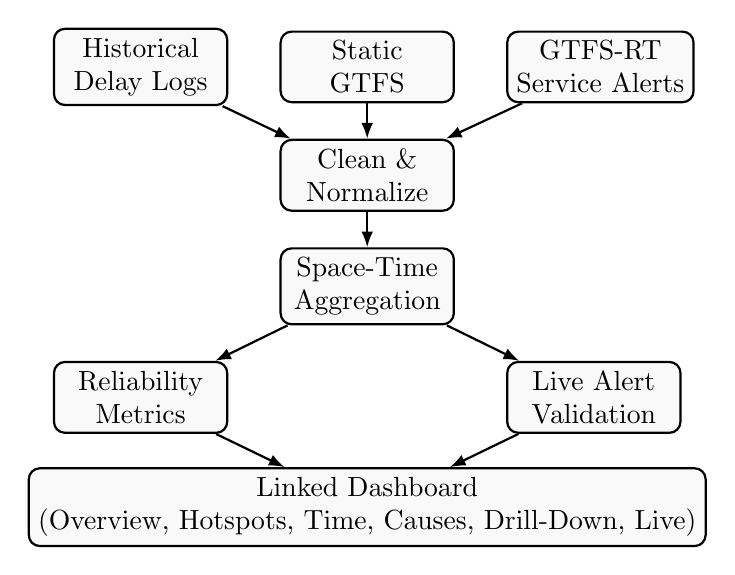
\begin{tikzpicture}[
    node distance=0.45cm and 0.65cm,
    box/.style={
        rectangle,
        rounded corners,
        draw=black,
        thick,
        align=center,
        minimum width=2.2cm,
        minimum height=0.8cm,
        fill=gray!5
    },
    arrow/.style={
        -{Latex[length=2mm]},
        thick
    }
]

\node[box] (hist) {Historical\\Delay Logs};
\node[box, right=of hist] (gtfs) {Static\\GTFS};
\node[box, right=of gtfs] (alerts) {GTFS-RT\\Service Alerts};

\node[box, below=of gtfs] (clean) {Clean \&\\Normalize};
\node[box, below=of clean] (agg) {Space-Time\\Aggregation};
\node[box, below left=of agg] (metrics) {Reliability\\Metrics};
\node[box, below right=of agg] (validation) {Live Alert\\Validation};

\node[box, below=1.8cm of agg] (dash) {Linked Dashboard\\(Overview, Hotspots, Time, Causes, Drill-Down, Live)};

\draw[arrow] (hist) -- (clean);
\draw[arrow] (gtfs) -- (clean);
\draw[arrow] (alerts) -- (clean);
\draw[arrow] (clean) -- (agg);
\draw[arrow] (agg) -- (metrics);
\draw[arrow] (agg) -- (validation);
\draw[arrow] (metrics) -- (dash);
\draw[arrow] (validation) -- (dash);

\end{tikzpicture}
\caption{TTC Pulse data-analytics architecture: ingestion, canonicalization, aggregation, reliability scoring, and live-alert validation feeding the dashboard.}
\label{fig:ttc-architecture}
\end{figure}

\subsection{Data-Analytics Methodology}
\textbf{Data preparation and normalization.}
Historical delay events are transformed into a canonical event structure with service date/time, mode, route or station context, incident category, and operational measures (\texttt{Min Delay}, \texttt{Min Gap}). GTFS dimensions are used as a reference layer to standardize route/station identity and preserve consistency across analytical views.

\textbf{Spatiotemporal analysis design.}
We aggregate by entity and time to answer ``where'', ``when'', and ``how often'' disruptions recur. Temporal views include yearly, monthly, weekday, and hour-bin slices. This is appropriate for TTC reliability because recurrence patterns are strongly schedule- and period-dependent.

\textbf{Reliability metric framework.}
For each entity $u$ in time window $t$, we compute:
\begin{itemize}
    \item \textbf{Frequency} ($F$): total disruption-event volume in the entity-time slice (implemented as summed \texttt{event\_count}/\texttt{frequency}); here, an \emph{incident} means one recorded delay/disruption event tied to a service date and incident category
    \item \textbf{Severity} ($\mathrm{Sev}_{90}$): upper-tail delay behavior (90th-percentile delay minutes)
    \item \textbf{Regularity} ($\mathrm{Reg}_{90}$): upper-tail gap/headway irregularity (90th-percentile gap minutes)
    \item \textbf{Cause Mix} ($C$): disruption cause composition signal
\end{itemize}

Cause mix is computed from category concentration:
\[
C(u,t)=1-\sum_{k} p_k(u,t)^2,
\]
where $p_k$ is the share of category $k$ within entity-time slice $(u,t)$.

For ranking, we use the implemented composite formula:
\[
S(u,t)=0.35\,z(F)+0.30\,z(\mathrm{Sev}_{90})+0.20\,z(\mathrm{Reg}_{90})+0.15\,C.
\]
The z-score normalization for each metric $x$ is:
\[
z(x)=\frac{x-\mu_x}{\sigma_x},
\]
computed within the peer comparison set (same mode/date-window context). If $\sigma_x=0$, the implementation safely falls back to zero contribution for that standardized term. The dashboard always exposes component metrics beside the composite score.

Interpretation of $S(u,t)$ is relative (not bounded to $[-1,1]$):
\begin{itemize}
    \item $S(u,t)>0$: worse-than-peer reliability profile in the selected comparison set
    \item $S(u,t)<0$: better-than-peer reliability profile in the selected comparison set
    \item $S(u,t)\approx 0$: near peer-average reliability profile
\end{itemize}
Larger absolute magnitude means stronger deviation from peer-average behavior.

\subsection{Data-Analytics Architecture}
The implementation follows a local-first layered architecture:
\begin{itemize}
    \item \textbf{Raw/Bronze}: ingestion and lineage-preserving storage
    \item \textbf{Silver}: canonical dimensions, bridges, review queues, normalized facts
    \item \textbf{Gold}: stakeholder marts for reliability metrics, rankings, temporal profiles, and alert validation
\end{itemize}

Runtime stack:
\begin{itemize}
    \item \textbf{Storage/Query}: DuckDB + Parquet
    \item \textbf{Serving}: Streamlit dashboard
    \item \textbf{Live capture}: GTFS-RT service-alert sidecar scheduled every 30 minutes (local OS scheduler)
\end{itemize}

\textbf{Why we shifted from Airflow to local OS scheduling.}
Based on course-scope guidance discussed with the instructor (keep deployment reproducible on student laptops and avoid server-grade operational dependencies), we moved from Airflow-first orchestration to local OS-native scheduling (\texttt{launchd} on macOS and Task Scheduler on Windows). The key reasons were:
\begin{itemize}
    \item only one recurring production task was needed (30-minute alert sidecar cycle)
    \item Airflow introduces extra runtime services (scheduler/webserver/metadata DB) that are disproportionate for this scope
    \item local schedulers improve teammate portability and reduce setup/maintenance overhead
    \item this choice preserves focus on analytics quality rather than infrastructure operations
\end{itemize}
Airflow DAGs are retained as legacy/reference artifacts, but active execution for this project milestone is local-first.
\textbf{Scope expansion note:} streetcar support has started at the data-model level and will be integrated into reliability marts and dashboard views in the next phase.

\subsection{Algorithms and Implemented Components}
\textbf{(1) Canonicalization strategy.}
Bus analytics use route-first canonicalization and subway analytics use station-first canonicalization. Ambiguous/unmatched mappings are retained in review-oriented tables instead of being silently dropped.

\textbf{(2) Windowed ranking aggregation.}
For selected service-date windows, rankings are recomputed from metrics marts using windowed aggregation and rank ordering on composite score (with frequency as tie-break context).

\textbf{(3) Alert-hotspot alignment metric design (planned KPI, partial implementation).}
Let $A$ be the set of live alerts in a validation window and let $H_K$ be the historical top-$K$ hotspots from the selected baseline window. The evaluation metrics are:
\[
\mathrm{HitRate}=\frac{1}{|A|}\sum_{a \in A}\mathbf{1}[a \in H_K],
\qquad
\mathrm{Lift}=\frac{\mathrm{HitRate}}{\mathrm{BaselineHitRate}}.
\]
where \(\mathrm{BaselineHitRate}\) is computed against a non-hotspot baseline set of equal size (or a random baseline under the same selector constraints).

Interpretation for stakeholders:
\begin{itemize}
    \item \textbf{HitRate}: ``Of all current live alerts, what fraction fall in historically high-risk hotspots?''
    \item \textbf{Lift}: ``How much better is hotspot targeting than a baseline expectation?''
    \item \(\mathrm{Lift}>1\): live alerts are more concentrated in historical hotspots than baseline (supports recurrence claim)
    \item \(\mathrm{Lift}\approx 1\): hotspot concentration is similar to baseline (weak validation)
    \item \(\mathrm{Lift}<1\): historical hotspots do not explain current live alerts well in that window
\end{itemize}
This directly supports the TTC Pulse storyline by testing whether ``today's disruptions'' align with ``historically recurring hotspots''.

Current implementation status at midterm: the dashboard currently surfaces alert-match status and selector-validity diagnostics in the Live Alert Alignment page, while explicit \(\mathrm{HitRate}\)/\(\mathrm{Lift}\) KPIs are specified and ready for the evaluation stage.

\subsection{Limitations}
\begin{itemize}
    \item Cause-mix signal is less stable in very fine-grain slices.
    \item GTFS-RT selector sparsity can reduce exact entity-match confidence.
    \item Spatial certainty is stronger for canonical subway stations than for bus route-centroid approximations.
    \item Composite ranking interpretation requires component-metric visibility to avoid over-reliance on a single score.
\end{itemize}


\section{Evaluation and Results}

\subsection{Evaluation Introduction}
At midterm, evaluation focuses on two goals: (1) verify that implemented metrics and dashboard slices recover meaningful recurring reliability patterns, and (2) document what is already operational versus deferred to final evaluation (notably explicit HitRate/Lift KPI reporting).

\subsection{Datasets and Summary Statistics}
Current analysis uses:
\begin{itemize}
    \item \textbf{TTC Bus Delay Data (2014--2026 Jan)}~\cite{toronto_ttc_bus_delay_data}
    \item \textbf{TTC Subway Delay Data (2014--2026 Jan)}~\cite{toronto_ttc_subway_delay_data}
\end{itemize}
These contain timestamped incident rows with route/line context, delay minutes (\texttt{Min Delay}), gap minutes (\texttt{Min Gap}), and incident categories.

Observed summary statistics for the current midterm window:
\begin{itemize}
    \item \textbf{145 months} of observations
    \item \textbf{Average incident frequency}: 5,354 events/month
    \item \textbf{Average delay severity (P90)}: 18.71 minutes
    \item \textbf{Average regularity irregularity (P90 Min Gap)}: 29.94 minutes
\end{itemize}

\subsection{Preliminary Empirical Patterns}
\begin{figure}[t]
    \centering
    \includegraphics[width=\linewidth]{image/ttc_reliability}
    \caption{Temporal evolution of TTC bus reliability metrics (2014--2026), showing monthly incident frequency and P90 delay severity.}
    \label{fig:ttc-reliability-trend}
\end{figure}

Figure~\ref{fig:ttc-reliability-trend} shows structured temporal recurrence rather than random fluctuation. A dip appears during 2020--2021, with elevated stabilization in later years.

\begin{figure}[t]
    \centering
    \includegraphics[width=\linewidth]{image/hotspot_bus_route}
    \caption{Top bus routes ranked by composite reliability score in the selected analysis window.}
    \label{fig:ttc-route-hotspots}
\end{figure}

Figure~\ref{fig:ttc-route-hotspots} indicates concentration of disruption risk in a small subset of routes, supporting hotspot-focused intervention logic.

\subsection{What Is Implemented vs Deferred}
\textbf{Implemented at midterm:}
\begin{itemize}
    \item date-windowed bus/subway reliability marts and rankings
    \item recurring hotspot and drill-down dashboard workflow
    \item live alert ingestion sidecar (30-minute local scheduler)
    \item live alert selector/match-status diagnostics in dashboard
\end{itemize}

\textbf{Deferred to final evaluation:}
\begin{itemize}
    \item explicit HitRate and Lift KPI publication in results tables/charts
    \item baseline design sensitivity checks and statistical significance analysis
    \item completed streetcar integration in marts and dashboard
\end{itemize}

\subsection{Implications}
Even at midterm, results support a key operational implication: reliability issues are localized and recurring, so targeted route/station-time interventions are likely more effective than system-wide uniform actions.

\section{Conclusion}
This midterm milestone delivers the core TTC reliability analytics foundation: integrated data pipeline, interpretable metric framework, composite ranking, and stakeholder-facing dashboard with live-alert diagnostics. The project has moved beyond proposal stage into an operational analytics system.

Final-phase work will complete formal live-validation KPIs (HitRate/Lift), expand streetcar coverage, and strengthen statistical robustness and reporting synthesis.

\vspace{-0.5em}
\bibliographystyle{ACM-Reference-Format}
\bibliography{midterm_refs}
\nocite{*}

\end{document}
